\section{Color representations}
While demosaiced RGB data is commonly used and convenient for many tasks, there are often alternative color representations that are better suited for specific purposes.
In many cases, the luminance (brightness) of each pixel is more crucial than the chrominance (color).
For many computer vision tasks, like Licas-Kanade method, the chrominance is not used at all \cite{lucasIterativeImageRegistration1981}.

\subsection{YCbCr}
A commonly used color representation in digital images is YCbCr
\footnote{In the computer industry, the term YUV is widely used to refer to colorspaces that are encoded using YCbCr.}
, which separates the luminance and chrominance components, as depicted in Figure \ref{fig:ycbcr_example}.
In the YCbCr color space, the Y component represents the luminance or brightness of the pixel, while the Cb and Cr components represent the blue-difference and red-difference chrominance information, respectively.

\begin{figure}[H]
    \centering
    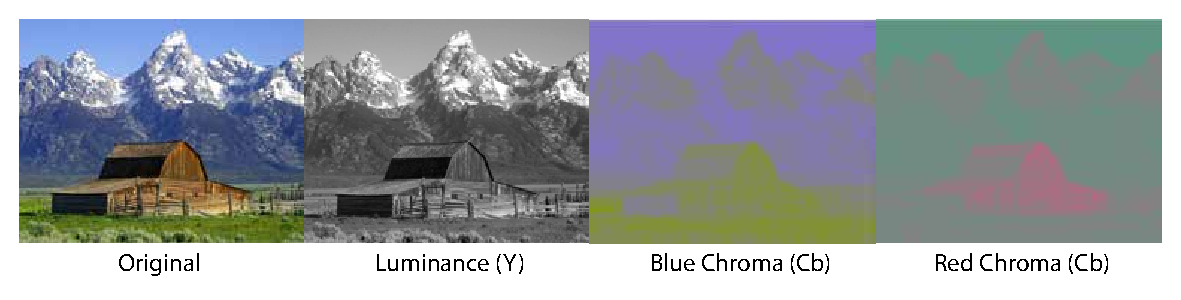
\includegraphics[width=\textwidth]{figures/debayer/YCbCr_example.pdf}
    \caption{Visualization of channels in a YCbCr image \cite{photoEnglishJohnMoulton2004}.}
    \label{fig:ycbcr_example}
\end{figure}

\subsubsection{Chroma subsampling}
One important property of the YCbCr color space is that it enables chroma subsampling, which is a technique used to reduce the amount of data required to represent an image while preserving visual fidelity \cite{ChromaSubsampling2023}.

Chroma subsampling involves sampling the chrominance components (Cb and Cr) at a lower resolution compared to the luminance component (Y).
A commonly used subsampling scheme is 4:2:0, where the chrominance components are sampled at half the resolution of the luminance component in both the horizontal and vertical directions \cite{ChromaSubsampling2023}.

\begin{figure}[H]
    \centering
    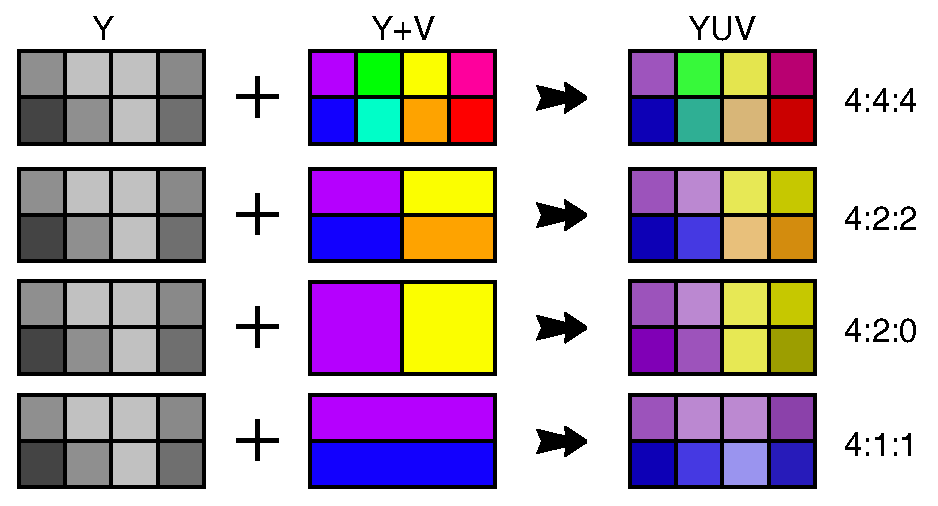
\includegraphics[width=.8\textwidth]{figures/debayer/chroma_subsampling.pdf}
    \caption{Chroma subsampling \cite{stevo-88EnglishMostWidely2010}.}
    \label{fig:ycbcr_example}
\end{figure}

As the human eye is more sensitive to changes in luminance compared to chrominance, chroma subsampling is particularly useful for maintaining visual fidelity during compression \cite{lambWhyRodsCones2016}.
It is important to note that for computer vision applications, this is not necessarily the case.

Still, when chroma subsampling can be reasonable when used on debayered images, as they contain a lot of redundant information from the debayering process, as every pixel contains three color channels insted of the single one in the bayer image.


\subsection{Analog legacy}
A final note on color representations is that several color formats that are still still affected by analog legacy.
For instance, the BT.601, which ais a variant of YCbCr only use values from 16 to 235 for the Y component and 16 to 240 for the Cb and Cr components \cite{YCbCr2023}.
The remaining space is called headroom and footroom used to accomodate transient signals such as filter overshoots \cite{Rec6012023}.


